\documentclass[a4paper, top=10mm]{article}
%for writing from the top
\usepackage{fullpage}
%for math
\usepackage{amsmath}
\usepackage{mathrsfs}
\usepackage{amsthm}
%for images
\usepackage{graphicx}
%for color
\usepackage{xcolor}
%for title
\title{\textbf{\huge{Animals Equations}}}
\author{Enigma n\textsuperscript{o}2}
\date{25\textsuperscript{th} June 2024}

\newtheorem*{hint}{Hint}

\addtolength{\voffset}{-2cm}
\addtolength{\textheight}{5cm}


\begin{document}
	\maketitle
	
	\vspace{1cm}
	
	\begin{center}
		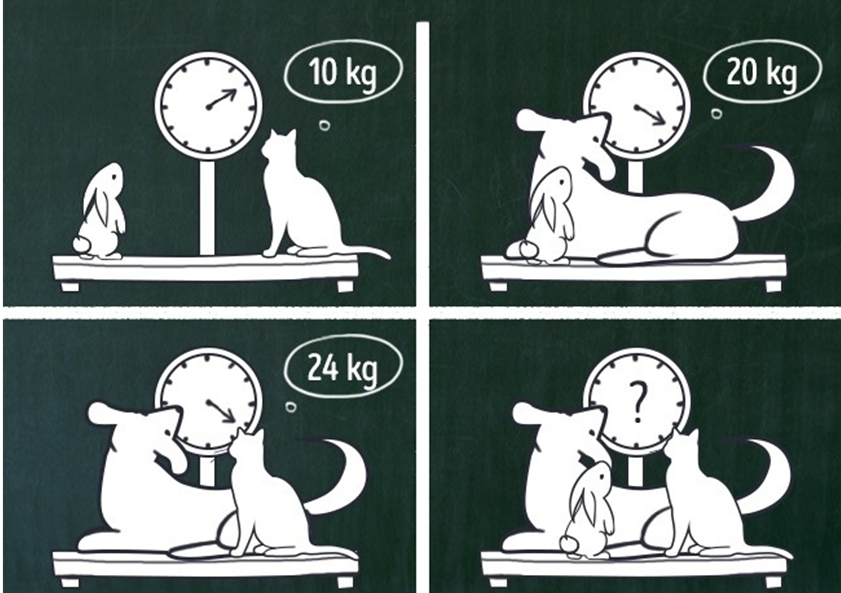
\includegraphics[width=\linewidth]{02image.png}\\
		What is the mass of the three animals combined?
	\end{center}
	
	% rabbit  = x
	% cat = y
	% dog = z
	%
	% x + y = 10
	% x + z = 20
	% y + z = 24
	%
	% z - y = 10
	% 2z = 34 => z = 17
	% so y = 7
	% and x = 3
	%
	% finally, x + y + z = 27kg
	
\end{document}